\section{Overview}
\label{sec:overview}

We begin with an overview of our approach to suggesting fixes for programs with
parse errors by fine-tuning error correcting parsers with prior knowledge of the
processes (novice) programmers follow to correct the errors.

\begin{figure}[ht]
\begin{ecode}
def foo(a):
  b = a + 42
  return b +
\end{ecode}

\begin{ecode}
def foo(a):
  b = a + 42
  return b + 17
\end{ecode}
\caption{(top) A Python program that adds an integer and returns it back that
has a parse error. (bottom) A possible fixed version with no parse errors.}
% TODO: Make it left-right instead of top-bottom.
\label{fig:foo-prog}
\end{figure}


\mypara{The Problem} Consider the simple program \texttt{foo} shown at the top
of \autoref{fig:foo-prog}. The program adds some number to the argument variable
\texttt{a} and tries to return it. However, there is an extra \texttt{+}
operator after the \texttt{return} statement. The extra \texttt{+} can either be
deleted or the programmer most likely intended to add another number like the
fix shown in the bottom of \autoref{fig:foo-prog}. This is a \emph{parse error}
and such parse errors can easily go unnoticed \citep{?} by programmers when they
are part of bigger programs.
%
Our goal is to use historical data of how programmers have fixed similar errors
in their programs to automatically and rapidly guide novices to come up with
candidate solutions like the one above.


\mypara{Solution: Error Correcting Parsers}
One approach to make such erroneous programs parse is to use \emph{Error
Correcting Parsers} (ECPs) \citep{?}. ECPs are based on \emph{dynamic
programming approaches} and have been used in recent literature to automatically
infer the intended parse tree for a program that doesn't belong to a certain
programming language, \ie a program that has a parse error. These dynamic
programming parsers have been used along side with \emph{error correcting
production rules} \citep{?} to generate a parse with the minimal edits from the
original program.

\mypara{Another Problem} However, these error-correcting parsers have a time
complexity that is cubed on the input program size and squared on the grammar
size used. And the biggest cost of these parsers is the large number of added
production rules. Therefore, they are not tractable or scalable options for
real-world programming languages and programs.


\mypara{Solution: Train classifier to predict error rules} The original Earley
parsing is a fairly efficient parsing algorithm \citep{?} based on dynamic
programming. Its error-correcting version is very inefficient though for larger
real-world grammars, since it requires the addition of a large number of error
production rules as mentioned before. However, not each erroneous program needs
all of those rules to be parsed. In this work, we present a novel strategy to
selecting just a small set of error production rules that can be used with an
updated \emph{Error Correcting Earley Parser} (ECEP) to repair a program with
parse errors.
%
To enable the efficient usage of a scalable ECEP we decompose the problem into 3
steps:
%
First, \emph{learn} the set of error productions rules each program with a parse
error needs from a corpus of fixed programs.
%
Second, \emph{predict}, for each erroneous program, a small set of error rules.
%
Third, \emph{parse} an erroneous program with the predicted rules and generate a
fix.
%
In the remainder of this section, we give a high-level overview
of our approach by describing how to:

\begin{enumerate}

  \item Use an \emph{Error Correcting Earley Parser} (ECEP) to repair programs
  with parse errors (\S~\ref{sec:overview:earleyparsing}),

  \item Abstract erroneous programs with theirs \emph{partial parses} by using
  Probabilistic Context-Free Grammars (PCFGs)
  (\S~\ref{sec:overview:abstraction}),

  \item Train \emph{sequence classifiers} on the abstracted programs to predict
  small sets of error production rules (\S~\ref{sec:overview:train}).

\end{enumerate}

\subsection{Background: Earley Parsing}
\label{sec:overview:earleyparsing}

\mypara{Earley Parsing} Earley parsing has been a touch-stone algorithm in the
history of parsing \citep{?}. An Earley parser is a chart parser that uses
dynamic programming, meaning that partial parses are stored in a data structure
called a chart, which can later be re-used. This eliminates backtracking and
prevents a combinatorial explosion. Worst case, it has a time complexity of
$O(n^3 G^2)$ for generic context-free grammars, where $n$ is the number of
\emph{tokens} of the input program and $G$ is the grammar size. However, this
parsing algorithm has limited use in large real-world programming languages, \eg
Python or Java, and more time- and memory-efficient parsing algorithms are used.
\autoref{fig:production-rules} presents for example some production rules for
the Python language. \emph{Terms} in the grammar starting with a capital letter
here represent non-terminal symbols while the rest are terminals that will
appear in a Python programs. The \texttt{Stmt} defines all the Python statements
for example.

\begin{figure}[ht]
\begin{ecode}
S -> Stmts_Or_Newlines Endmarker
...
Funcdef -> def Name Parameters : Suite
Suite -> Newline Indent Stmts_Or_Newlines Dedent
Stmts_Or_Newlines -> Stmt_Or_Newline | Stmt Stmts_Or_Newlines
Stmt -> Expr_Stmt | Pass_Stmt | Return_Stmt | Import_Stmt | ...
Return_Stmt -> return | return Arg_List
Arg_List -> Expr_Stmt | Expr_Stmt , Arg_List
...
\end{ecode}
\caption{Some production rules of the Python grammar}
\label{fig:production-rules}
\end{figure}

\begin{figure}[ht]
\begin{ecode}
Suite -> Err_Newline Err_Indent Stmts_Or_Newlines Err_Dedent
Return_Stmt -> ... | Err_Return | Err_Return Arg_List
Err_Return -> e | Err_Tag | H return
...
Err_Tag -> pass | raise | return | ...
...
InsertErr -> pass | raise | return | ...
...
newS -> S | S InsertErr
H -> H | H InsertErr
\end{ecode}
\caption{Error production rules for the Python grammar presented in
\autoref{fig:production-rules}}
\label{fig:error-rules}
\end{figure}

\mypara{Error Correcting Parsing} Recent work has presented an \emph{Error
Correcting Earley Parser} (ECEP) \citep{?}, which extends the original
algorithm's operations, with the goal to find a minimum-edit parse for a program
with parse errors. The ECEP also extends the original grammar $G$ with a set of
\emph{error production rules} to create a new \emph{error grammar} $G'$. This
grammar contains error rules for the three major types of errors that this
algorithm considers, \ie it adds error rules for all terminals that account for
\emph{insertion}, \emph{deletion}, \emph{replacement} errors.
\autoref{fig:error-rules} presents \texttt{Err\_Return} that add these rules for
the terminal \texttt{return}.

It also adds some non-terminal error rules that introduce these errors when the
parsing algorithm is executed. These rules are for example in lines 1 and 2 of
\autoref{fig:error-rules}. Therefore, the new and larger error correcting
grammar $G'$ is introduced that is at least 3 times larger than $G$, making ECEP
not scalable for large programs or programs with a lot of parse errors.

However, ECEP is an effective approach on finding minimum distance parses for
programs than don't belong into the given programming language, \ie have parse
errors. A straight-forward approach is to keep ECEP tractable is to only add a
small set of error production rules, \ie keep the size of $G'$ limited and
slightly larger than the original grammar $G$.

% Our notion of a fix is defined as a \emph{replacement} of an existing expression
% with a new \emph{candidate} expression at a specific program location. For
% example, the \mbd program is fixed by replacing |(hd * i)| with the expression
% |[hd * i]| on line 4. We focus on AST-level replacements as they are compact yet
% expressive enough to represent fixes.


% \mypara{Generic Abstract Syntax Trees}
% %
% We represent the different possible candidate expressions via abstract fix
% templates called \emph{Generic Abstract Syntax Trees} (GAST) which each
% correspond to many possible expressions.
% %
% GASTs are obtained from concrete ASTs in two steps.
% %
% First, we abstract concrete variable, function, and operator names.
% %
% Next, we prune GASTs at a certain depth $d$ to keep only the top-level changes
% of the fix. Pruned sub-trees are replaced with \emph{holes}, which can represent
% \emph{any} possible expression in our language.


% Together, these steps ensure that GASTs only contain information about a fix's
% \emph{structure} rather than the specific changes in variables and functions.
% %
% For example, the fix |[hd * i]| in the \mbd example is represented by the GAST
% of the expression |[_ $\oplus$ _]|, where variables |hd| and |i| are abstracted
% into holes (\eg by pruning the GAST at a depth $d=2$) and |*| is represented by
% an abstract binary operator |$\oplus$|. Our approach is similar to that of
% Lerner \emph{et al.}~\citep{Lerner2007-dt}, where AST-level modifications are
% used, however, our proposed GASTs represent more abstract fix schemas.


\subsection{Abstracting program token sequences}
\label{sec:overview:abstraction}

\begin{figure}[ht]
\begin{ecode}
def Name ( Name ) : Newline
Indent Name = Name + Number Newline
return Name + Newline
Dedent End_Marker
\end{ecode}

\begin{ecode}
def Name Parameters : Newline
Indent Small_Stmt Newline
return Arith_Expr Arith_Op Newline
Dedent End_Marker
\end{ecode}
\caption{(top) The token sequence generated by the lexer for the program at
\autoref{fig:foo-prog}. (bottom) The abstracted token sequence for the same
program.}
\label{fig:foo-prog-abstract}
\end{figure}

We need to work on programs that have parse errors, \ie we can not generate a
parse tree for them to perform all kinds of analyses that have been used in
previous work on automated program repair \citep{?} and program analysis in
general \citep{?}.
%
The highest form of abstraction that we can use is the output of the
\emph{lexer}. The lexer tokenizes the program and returns a program \emph{token
sequence} with some form of abstractions, \eg no variable names, defining the
underlying statement blocks \etc, as shown in \autoref{fig:foo-prog-abstract}.
This token sequence is appropriate for training our sequence classifier models,
but as we will show later on, they can contain a lot of irrelevant context for
the parse error at hand and can lead to very large sequences for our models.

\mypara{Solution: Abstract with partial parses} A \emph{parser} will hold some
internal state of the partial parses it has generated until a parse error is
encountered. The parser will then fail and return an error pointing to the
location that lead to that parse error. However, these partial parses provide
useful information and abstraction for the program at hand. For example, the
partial parse tree shown in \autoref{fig:partial-parse-tree} can be generated by
an Earley parser for the running example program. Using this partial parse tree
we get the \emph{abstracted token sequence} shown in the bottom of
\autoref{fig:foo-prog-abstract}. Any \emph{completed} production rule, \ie the
one for \texttt{Parameters}, can be used to replace the relevant non-terminals,
\ie the parenthesis with the function arguments, with the high-level
non-terminal.

\begin{figure}
    \centering
    \begin{tikzpicture}
    [font=\small, edge from parent,
    every node/.style={top color=white, bottom color=black!15,
    circle, minimum size=11mm, draw=black!75,
    thick, drop shadow, align=center},
    edge from parent/.style={draw=black!75,thick},
    level distance=1.6cm, xscale=1.3]
    \node (func) {Funcdef}
        child {
            node (def) {\texttt{\bfseries def}}
        }
        child {
            node (name1) {\texttt{Name}}
        }
        child {
            node (params) {\texttt{Params}}
            child {
                node (openParen) {\texttt{\bfseries (}}
            }
            child {
                node (name2) {\texttt{Name}}
            }
            child {
                node (closeParen) {\texttt{\bfseries )}}
            }
        }
        child {
            node (colon) {\texttt{\bfseries :}}
        }
        child [level distance=0.3cm, xscale=1.35] {
            node  (suite) {\texttt{Suite}}
            child [level distance=1.3cm] {
                node (etc) {\texttt{...}}
            }
            child [level distance=1.3cm] {
                node (RetStmt) {\texttt{RetStmt}}
                % node (RetStmt) {\texttt{\begin{tabular}{c}
                %                                 Return\\
                %                                 Stmt
                %                             \end{tabular}}}
                child {
                    node (return) {\texttt{\bfseries return}}
                }
                child {
                    node (ArgList) {\texttt{ArgList}}
                    child [level distance=1.6cm] {
                        node (ArExpr1) {\texttt{ArExpr}}
                        child [level distance=1.3cm] {
                            node (ArExpr2) {\texttt{Literal}}
                        }
                        child [level distance=1.3cm] {
                            node (plus) {\texttt{\bfseries +}}
                        }
                    }
                }
            }
        };
    \end{tikzpicture}
    \caption{The partial parse tree generated for the example at \autoref{fig:orig-prog}}
    \label{fig:partial-parse-tree}
\end{figure}


\begin{figure}
    \centering
    \begin{minipage}[t]{0.28\linewidth}
        \centering
        \resizebox{!}{0.25\textheight}{
        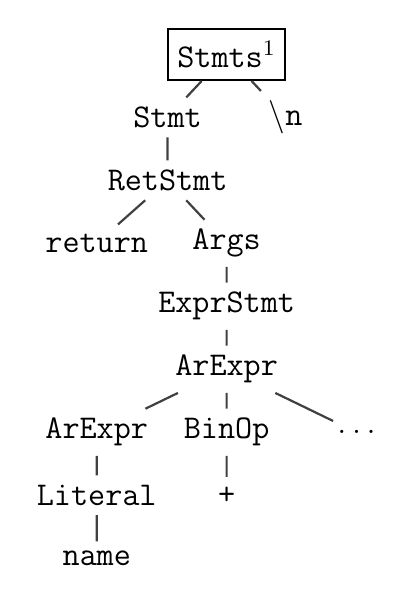
\begin{tikzpicture}
        [font=\large, edge from parent,
        % every node/.style={top color=white, bottom color=black!20,
        % ellipse, minimum size=8mm, draw=black!75,
        % thick, drop shadow, align=center},
        edge from parent/.style={draw=black!75, thick},
        level distance=0.8cm, xscale=1.0]
        \node [style={minimum size=6.5mm, draw=black, thick}] (stmts2) {\texttt{Stmts$^1$}}
        child {
            node (stmt2) {\texttt{Stmt}}
            child {
                node (RetStmt) {\texttt{RetStmt}}
                child [xscale=1.2] {
                    node (return) {\texttt{\bfseries return}}
                }
                child {
                    node (args) {\texttt{Args}}
                    child {
                        node (expr2) {\texttt{ExprStmt}}
                        child [xscale=1.1] {
                            node (arexpr1) {\texttt{ArExpr}}
                            child {
                                node (arexpr2) {\texttt{ArExpr}}
                                child {
                                    node (literal) {\texttt{Literal}}
                                    child {
                                        node (name3) {\texttt{name}}
                                    }
                                }
                            }
                            child {
                                node (binop) {\texttt{BinOp}}
                                child {
                                    node (plus) {\texttt{\bfseries +}}
                                }
                            }
                            child {
                                node (empty) {\texttt{$\dots$}}
                            }
                        }
                    }
                }
            }
        }
        child {
            node (newline3) {\texttt{\textbackslash n}}
        };
        \end{tikzpicture}
        } \subcaption{The partial parse tree for the example at
        \autoref{fig:bad-prog}.}
        \label{fig:partial-parse-tree-2}
    \end{minipage}
    \hspace{0.02\linewidth}%
    \begin{minipage}[t]{0.35\linewidth}
        \centering
        \hspace*{0.04\linewidth}%
        \resizebox{!}{0.25\textheight}{
            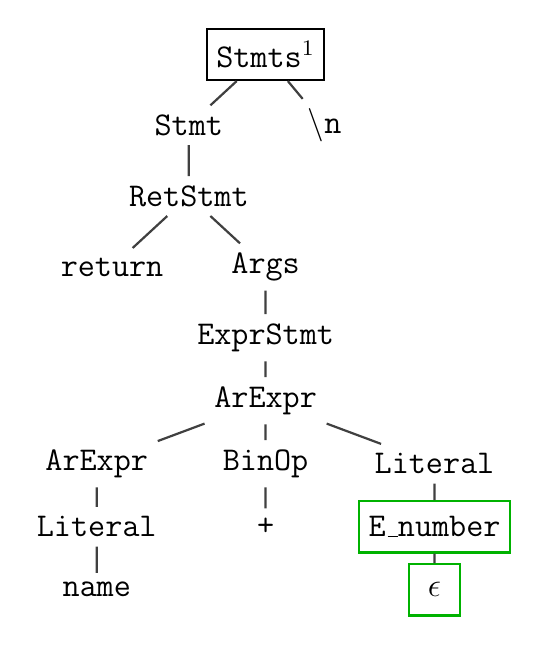
\begin{tikzpicture}
            [font=\large, edge from parent,
            % every node/.style={top color=white, bottom color=black!20,
            % ellipse, minimum size=8mm, draw=black!75,
            % thick, drop shadow, align=center},
            edge from parent/.style={draw=black!75, thick},
            level distance=0.9cm, xscale=1.0]
            \node [style={minimum size=6.5mm, draw=black, thick}] (stmts2) {\texttt{Stmts$^1$}}
            child [xscale=1.3] {
                node (stmt2) {\texttt{Stmt}}
                child {
                    node (RetStmt) {\texttt{RetStmt}}
                    child {
                        node (return) {\texttt{\bfseries return}}
                    }
                    child {
                        node (args) {\texttt{Args}}
                        child {
                            node (expr2) {\texttt{ExprStmt}}
                            child [level distance=0.8cm, xscale=1.1] {
                                node (arexpr1) {\texttt{ArExpr}}
                                child {
                                    node (arexpr2) {\texttt{ArExpr}}
                                    child {
                                        node (literal1) {\texttt{Literal}}
                                        child {
                                            node (name3) {\texttt{name}}
                                        }
                                    }
                                }
                                child {
                                    node (binop) {\texttt{BinOp}}
                                    child {
                                        node (plus) {\texttt{\bfseries +}}
                                        }
                                }
                                child {
                                    node (literal2) {\texttt{Literal}}
                                    child {
                                        node [style={minimum size=6.5mm, draw=black!30!green, thick}] (enumber) {\texttt{E\_number}}
                                        child {
                                            node [style={minimum size=6.5mm, draw=black!30!green, thick}] (eps) {\texttt{$\epsilon$}}
                                        }
                                    }
                                }
                            }
                        }
                    }
                }
            }
            child {
                node (newline3) {\texttt{\textbackslash n}}
            };
            \end{tikzpicture}
        } \subcaption{Adding a number with the green \texttt{E\_number} error rule.}
        \label{fig:adding-partial}
    \end{minipage}
    \hspace{0.01\linewidth}%
    \begin{minipage}[t]{0.32\linewidth}
        \centering
        \resizebox{!}{0.25\textheight}{
            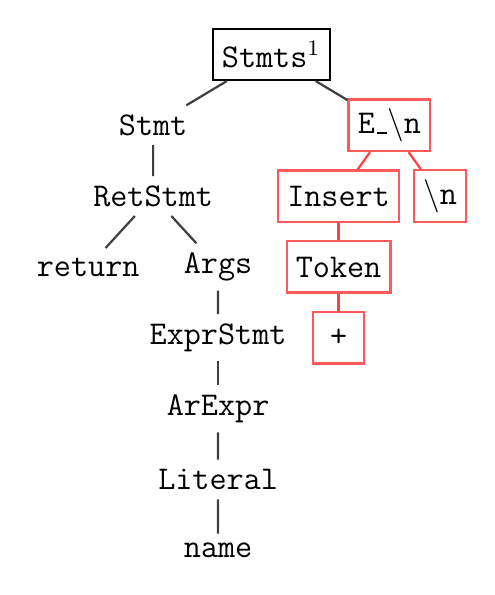
\begin{tikzpicture}
            [font=\large, edge from parent,
            % every node/.style={top color=white, bottom color=black!20,
            % ellipse, minimum size=8mm, draw=black!75,
            % thick, drop shadow, align=center},
            edge from parent/.style={draw=black!75, thick},
            level distance=0.9cm, xscale=2.0]
            \node [style={minimum size=6.5mm, draw=black, thick}] (stmts2) {\texttt{Stmts$^1$}}
            child {
                node (stmt2) {\texttt{Stmt}}
                child [xscale=0.55] {
                    node (RetStmt) {\texttt{RetStmt}}
                    child {
                        node (return) {\texttt{\bfseries return}}
                    }
                    child {
                        node (args) {\texttt{Args}}
                        child {
                            node (expr2) {\texttt{ExprStmt}}
                            child {
                            node (arexpr1) {\texttt{ArExpr}}
                                child {
                                    node (literal1) {\texttt{Literal}}
                                    child {
                                        node (name3) {\texttt{name}}
                                    }
                                }
                            }
                        }
                    }
                }
            }
            child {
                node [style={minimum size=6.5mm, draw=red!65, thick}] (enewline) {\texttt{E\_\textbackslash n}}
                child [edge from parent/.style={draw=red!75, thick}, xscale=0.43] {
                    node [style={minimum size=6.5mm, draw=red!65, thick}] (insert) {\texttt{Insert}}
                    child {
                        node [style={minimum size=6.5mm, draw=red!65, thick}] (token) {\texttt{Token}}
                        child {
                            node [style={minimum size=6.5mm, draw=red!65, thick}] (plus) {\texttt{\bfseries +}}
                        }
                    }
                }
                child [edge from parent/.style={draw=red!75, thick}, xscale=0.43] {
                    node [style={minimum size=6.5mm, draw=red!65, thick}] (newline3) {\texttt{\textbackslash n}}
                }
            };
            \end{tikzpicture}
        }
        \subcaption{Deleting the \texttt{+} with red \texttt{E\_\textbackslash n} error rule.}
        \label{fig:deleting-partial}
    \end{minipage}
    \caption{The rest of the problematic function in
    \autoref{fig:partial-parse-tree-1} and two possible error-correcting parses}
    \label{fig:two-partial-parses}
\end{figure}


\mypara{Probabilistic Context-Free Grammars} Even if the original grammar $G$ is
not ambiguous, generating partial parses can be ambiguous. Earley parsing is an
dynamic programming technique and internally keeps all possible parses from the
begging of the token sequence until position $i$ in its charts. Therefore, when
there is a parse error at token $i$, it is possible to have more than one
partial parses to choose from in order to generate the abstracted token
sequence.

In that aid, Probabilistic Context-Free Grammars (PCFGs) have been used in
previous work \citep{?} to select \emph{complete} parses for ambiguous grammars.
A PCFG associates each of its production rules with a \emph{weight} or
\emph{probability}. Each parse tree that is generated during parsing is also
associated with a probability. Finally, the one with the highest probability is
selected as a final parse tree. A PCFG can simply be learned \citep{?} by
counting the production rules used to parse a number of programs belonging to
that language for each terminal token.

We apply this approach to select a partial parse from the Earley parser. The
probabilities can again be learned from the \emph{fixed} programs of a large
corpus of erroneous and fixed programs. The selected partial parse can then be
used to generate an abstracted token sequence.


\subsection{Training Sequence Classifiers}
\label{sec:overview:train}
The abstracted token sequences we extracted from the partial parses present us
with small abstracted sequences that maintain a lot of the program's context
along with some hints of the user's intended behavior for the program due to the
PCFG usage. Additionally, recent work on machine learning, and especially on
Natural Language Processing (NLP) \citep{?}, have utilized \emph{sequence
models} to learn underlying patterns in their data. These models stand out in
domains where the input is a sequence and feature extraction methods are not
readily available to utilize in order to use the older classic neural network
models \citep{?}.

\mypara{Sequence models} Sequence-to-sequence (seq2seq) architectures aim to
transform a input sequence of tokens into a new sequence \citep{?}. These
architectures consist of an \emph{encoder} and a \emph{decoder}. The encoder
transforms the input token sequence into a \emph{$n$-dimensional abstract
vector} that captures all the essence and context of the input sequence. This
vector doesn't necessarily have some physical meaning and is just an internal
representation of the input sequence into a higher dimensional space. The
abstract vector is given as an input to the decoder, which in turn transforms it
into a output sequence. Both the encoder and the decoder can be an (older)
Long-Short-Term-Memory (LSTM)-based model \citep{?} or a state-of-the-art
\emph{Transformer} \citep{?}.

\mypara{Transformer Classifier} Next, we desire to train a model that can
correctly predict a small set of error production rules for a given abstracted
token sequence. We encode this problem into a \emph{supervised multi-class
classification}. A \emph{supervised} learning problem is one where, given a
labeled training set, the task is to learn a function that accurately maps the
inputs to output labels and generalizes to future inputs. In a
\emph{classification} problem, the function we are trying to learn maps inputs
to a discrete set of two or more output labels, called \emph{classes}.
Therefore, we encode the task of learning a function that will map token
sequences of erroneous programs to a small set of error production rules as a
\emph{multi-class} classification (MCC) problem. We use an \emph{encoder
transformer} to encode the input sequences into abstract vectors that we can
then feed into a \emph{Deep Neural Network (DNN)} classifier to train it and
make predictions.

\mypara{Predicting Error Rules via MCC}
Given a dataset of fixed parse errors, we can extract the small set of error
rules needed for each program to make it parse with an ECEP. We then train a
Transformer classifier on a new updated error-rule-labeled data set. Futhermore,
Neural networks have the advantage of associating each class with a
\emph{confidence score} that can be interpreted as the model's confidence of
each class being correct for a given input. Therefore, confidence scores can be
used to rank error rule predictions for new programs and select the top-$N$ ones
that will maintain a decent performance with the ECEP. Exploiting recent
advances in machine learning, we use deep and dense architectures
\citep{Schmidhuber_2015} for more accurate predictions.
